\documentclass{standalone}
\usepackage{tikz}
\usetikzlibrary{patterns, positioning}


\begin{document}
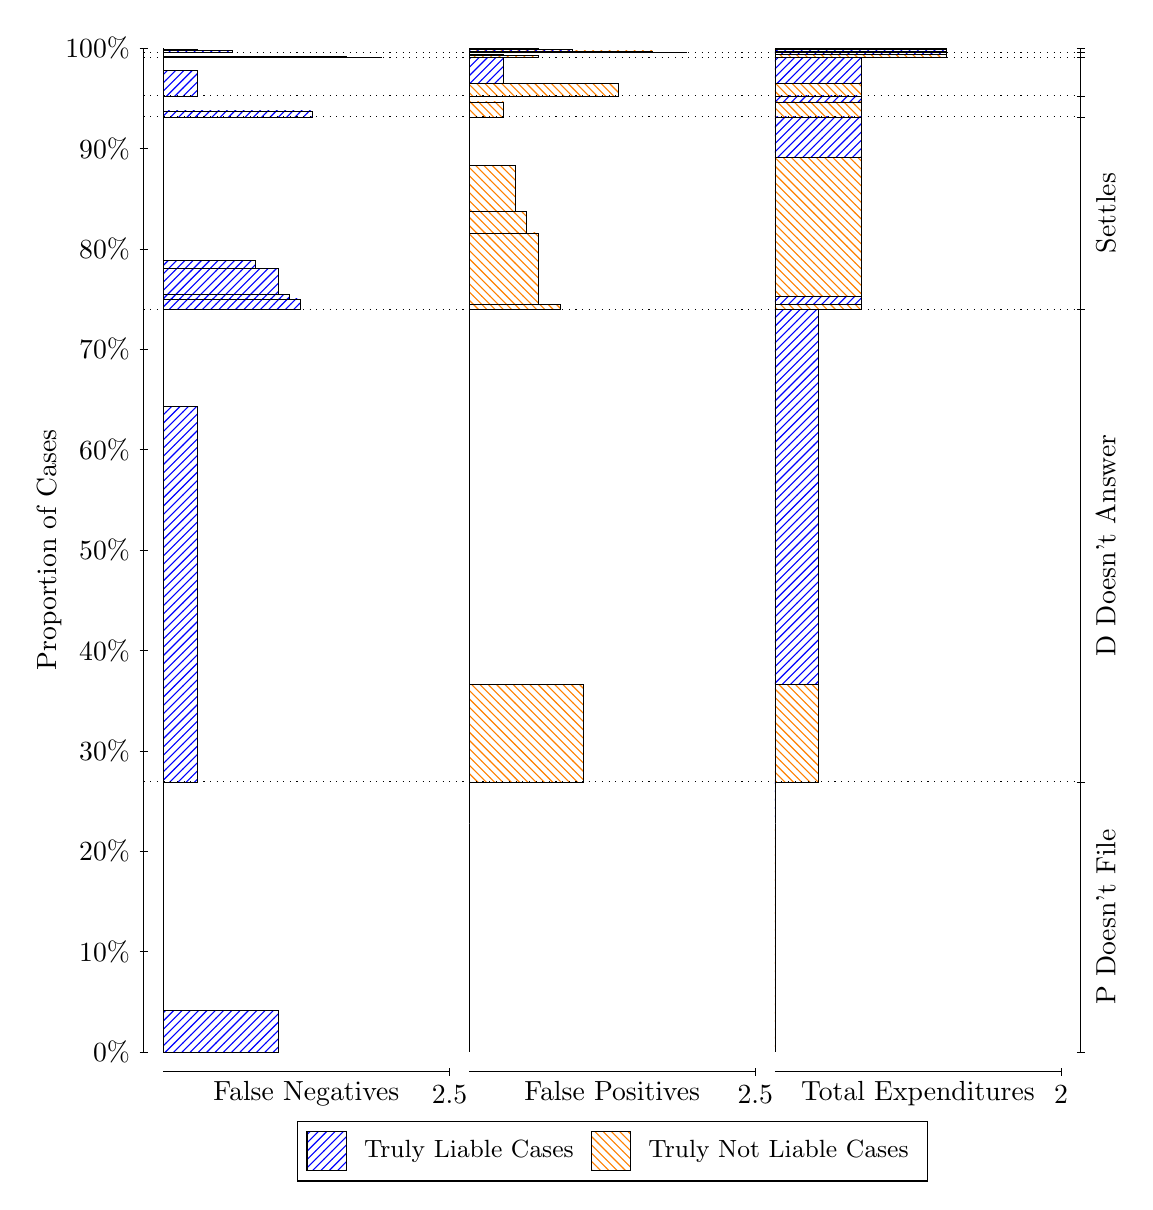
\begin{tikzpicture}
\draw[black, very thin] (1.5,1.75) -- (1.5,14.5);
\node[rotate=90, text=black, anchor=center] at (0.3, 8.125) {Proportion of Cases};
\draw[black, very thin] (1.45,1.75) -- (1.55,1.75);
\node[text=black, anchor=east] at (1.45, 1.75) {0\%};
\draw[black, very thin] (1.45,3.025) -- (1.55,3.025);
\node[text=black, anchor=east] at (1.45, 3.025) {10\%};
\draw[black, very thin] (1.45,4.3) -- (1.55,4.3);
\node[text=black, anchor=east] at (1.45, 4.3) {20\%};
\draw[black, very thin] (1.45,5.575) -- (1.55,5.575);
\node[text=black, anchor=east] at (1.45, 5.575) {30\%};
\draw[black, very thin] (1.45,6.85) -- (1.55,6.85);
\node[text=black, anchor=east] at (1.45, 6.85) {40\%};
\draw[black, very thin] (1.45,8.125) -- (1.55,8.125);
\node[text=black, anchor=east] at (1.45, 8.125) {50\%};
\draw[black, very thin] (1.45,9.4) -- (1.55,9.4);
\node[text=black, anchor=east] at (1.45, 9.4) {60\%};
\draw[black, very thin] (1.45,10.675) -- (1.55,10.675);
\node[text=black, anchor=east] at (1.45, 10.675) {70\%};
\draw[black, very thin] (1.45,11.95) -- (1.55,11.95);
\node[text=black, anchor=east] at (1.45, 11.95) {80\%};
\draw[black, very thin] (1.45,13.225) -- (1.55,13.225);
\node[text=black, anchor=east] at (1.45, 13.225) {90\%};
\draw[black, very thin] (1.45,14.5) -- (1.55,14.5);
\node[text=black, anchor=east] at (1.45, 14.5) {100\%};

\draw[black, very thin] (13.4,1.75) -- (13.4,14.5);
\draw[black, very thin] (13.35,1.75) -- (13.45,1.75);
\node[anchor=west] at (13.35, 1.75) {};
\draw[black, very thin] (13.35,5.1798) -- (13.45,5.1798);
\node[anchor=west] at (13.35, 5.1798) {};
\draw[black, very thin] (13.35,11.182) -- (13.45,11.182);
\node[anchor=west] at (13.35, 11.182) {};
\draw[black, very thin] (13.35,13.625) -- (13.45,13.625);
\node[anchor=west] at (13.35, 13.625) {};
\draw[black, very thin] (13.35,13.893) -- (13.45,13.893);
\node[anchor=west] at (13.35, 13.893) {};
\draw[black, very thin] (13.35,14.377) -- (13.45,14.377);
\node[anchor=west] at (13.35, 14.377) {};
\draw[black, very thin] (13.35,14.444) -- (13.45,14.444);
\node[anchor=west] at (13.35, 14.444) {};
\draw[black, very thin] (13.35,14.5) -- (13.45,14.5);
\node[anchor=west] at (13.35, 14.5) {};

\draw[black, very thin, pattern color=blue, pattern=north east lines] (1.75,1.75) rectangle (3.2033,2.2808);
\draw[black, very thin, pattern color=orange, pattern=north west lines] (1.75,2.2808) rectangle (1.75,5.1798);
\draw[black, very thin, pattern color=blue, pattern=north east lines] (1.75,5.1798) rectangle (2.186,9.9481);
\draw[black, very thin, pattern color=orange, pattern=north west lines] (1.75,9.9481) rectangle (1.75,11.182);
\draw[black, very thin, pattern color=blue, pattern=north east lines] (1.75,11.182) rectangle (3.494,11.313);
\draw[black, very thin, pattern color=blue, pattern=north east lines] (1.75,11.313) rectangle (3.3487,11.372);
\draw[black, very thin, pattern color=blue, pattern=north east lines] (1.75,11.372) rectangle (3.2033,11.699);
\draw[black, very thin, pattern color=blue, pattern=north east lines] (1.75,11.699) rectangle (2.9127,11.803);
\draw[black, very thin, pattern color=orange, pattern=north west lines] (1.75,11.803) rectangle (1.75,13.625);
\draw[black, very thin, pattern color=blue, pattern=north east lines] (1.75,13.625) rectangle (3.6393,13.703);
\draw[black, very thin, pattern color=orange, pattern=north west lines] (1.75,13.703) rectangle (1.75,13.893);
\draw[black, very thin, pattern color=blue, pattern=north east lines] (1.75,13.893) rectangle (2.186,14.215);
\draw[black, very thin, pattern color=orange, pattern=north west lines] (1.75,14.215) rectangle (1.75,14.377);
\draw[black, very thin, pattern color=blue, pattern=north east lines] (1.75,14.377) rectangle (4.5113,14.382);
\draw[black, very thin, pattern color=blue, pattern=north east lines] (1.75,14.382) rectangle (4.0753,14.398);
\draw[black, very thin, pattern color=orange, pattern=north west lines] (1.75,14.398) rectangle (1.75,14.444);
\draw[black, very thin, pattern color=blue, pattern=north east lines] (1.75,14.444) rectangle (2.622,14.466);
\draw[black, very thin, pattern color=blue, pattern=north east lines] (1.75,14.466) rectangle (2.186,14.479);
\draw[black, very thin, pattern color=orange, pattern=north west lines] (1.75,14.479) rectangle (1.75,14.5);
\draw[black, very thin, pattern color=orange, pattern=north west lines] (5.6333,1.75) rectangle (5.6333,4.649);
\draw[black, very thin, pattern color=blue, pattern=north east lines] (5.6333,4.649) rectangle (5.6333,5.1798);
\draw[black, very thin, pattern color=orange, pattern=north west lines] (5.6333,5.1798) rectangle (7.0867,6.4141);
\draw[black, very thin, pattern color=blue, pattern=north east lines] (5.6333,6.4141) rectangle (5.6333,11.182);
\draw[black, very thin, pattern color=orange, pattern=north west lines] (5.6333,11.182) rectangle (6.796,11.243);
\draw[black, very thin, pattern color=orange, pattern=north west lines] (5.6333,11.243) rectangle (6.5053,12.151);
\draw[black, very thin, pattern color=orange, pattern=north west lines] (5.6333,12.151) rectangle (6.36,12.429);
\draw[black, very thin, pattern color=orange, pattern=north west lines] (5.6333,12.429) rectangle (6.2147,13.005);
\draw[black, very thin, pattern color=blue, pattern=north east lines] (5.6333,13.005) rectangle (5.6333,13.625);
\draw[black, very thin, pattern color=orange, pattern=north west lines] (5.6333,13.625) rectangle (6.0693,13.815);
\draw[black, very thin, pattern color=blue, pattern=north east lines] (5.6333,13.815) rectangle (5.6333,13.893);
\draw[black, very thin, pattern color=orange, pattern=north west lines] (5.6333,13.893) rectangle (7.5227,14.055);
\draw[black, very thin, pattern color=blue, pattern=north east lines] (5.6333,14.055) rectangle (6.0693,14.377);
\draw[black, very thin, pattern color=orange, pattern=north west lines] (5.6333,14.377) rectangle (6.5053,14.404);
\draw[black, very thin, pattern color=orange, pattern=north west lines] (5.6333,14.404) rectangle (6.0693,14.423);
\draw[black, very thin, pattern color=blue, pattern=north east lines] (5.6333,14.423) rectangle (5.6333,14.444);
\draw[black, very thin, pattern color=orange, pattern=north west lines] (5.6333,14.444) rectangle (8.3947,14.449);
\draw[black, very thin, pattern color=orange, pattern=north west lines] (5.6333,14.449) rectangle (7.9587,14.465);
\draw[black, very thin, pattern color=blue, pattern=north east lines] (5.6333,14.465) rectangle (6.9413,14.478);
\draw[black, very thin, pattern color=blue, pattern=north east lines] (5.6333,14.478) rectangle (6.5053,14.5);
\draw[black, very thin, pattern color=orange, pattern=north west lines] (9.5167,1.75) rectangle (9.5167,4.649);
\draw[black, very thin, pattern color=blue, pattern=north east lines] (9.5167,4.649) rectangle (9.5167,5.1798);
\draw[black, very thin, pattern color=orange, pattern=north west lines] (9.5167,5.1798) rectangle (10.062,6.4141);
\draw[black, very thin, pattern color=blue, pattern=north east lines] (9.5167,6.4141) rectangle (10.062,11.182);
\draw[black, very thin, pattern color=orange, pattern=north west lines] (9.5167,11.182) rectangle (10.607,11.243);
\draw[black, very thin, pattern color=blue, pattern=north east lines] (9.5167,11.243) rectangle (10.607,11.346);
\draw[black, very thin, pattern color=orange, pattern=north west lines] (9.5167,11.346) rectangle (10.607,13.109);
\draw[black, very thin, pattern color=blue, pattern=north east lines] (9.5167,13.109) rectangle (10.607,13.625);
\draw[black, very thin, pattern color=orange, pattern=north west lines] (9.5167,13.625) rectangle (10.607,13.815);
\draw[black, very thin, pattern color=blue, pattern=north east lines] (9.5167,13.815) rectangle (10.607,13.893);
\draw[black, very thin, pattern color=orange, pattern=north west lines] (9.5167,13.893) rectangle (10.607,14.055);
\draw[black, very thin, pattern color=blue, pattern=north east lines] (9.5167,14.055) rectangle (10.607,14.377);
\draw[black, very thin, pattern color=orange, pattern=north west lines] (9.5167,14.377) rectangle (11.697,14.423);
\draw[black, very thin, pattern color=blue, pattern=north east lines] (9.5167,14.423) rectangle (11.697,14.444);
\draw[black, very thin, pattern color=orange, pattern=north west lines] (9.5167,14.444) rectangle (11.697,14.461);
\draw[black, very thin, pattern color=blue, pattern=north east lines] (9.5167,14.461) rectangle (11.697,14.482);
\draw[black, very thin, pattern color=orange, pattern=north west lines] (9.5167,14.482) rectangle (11.697,14.487);
\draw[black, very thin, pattern color=blue, pattern=north east lines] (9.5167,14.487) rectangle (11.697,14.5);
\draw[black, dotted] (1.5,5.1798) -- (13.4,5.1798);
\draw[black, dotted] (1.5,11.182) -- (13.4,11.182);
\draw[black, dotted] (1.5,13.625) -- (13.4,13.625);
\draw[black, dotted] (1.5,13.893) -- (13.4,13.893);
\draw[black, dotted] (1.5,14.377) -- (13.4,14.377);
\draw[black, dotted] (1.5,14.444) -- (13.4,14.444);
\draw[black, very thin] (1.75,1.5) -- (5.3833,1.5);
\node[text=black, anchor=north] at (3.5667, 1.5) {False Negatives};
\draw[black, very thin] (5.3833,1.45) -- (5.3833,1.55);
\node[text=black, anchor=north] at (5.3833, 1.45) {2.5};

\draw[black, very thin] (5.6333,1.5) -- (9.2667,1.5);
\node[text=black, anchor=north] at (7.45, 1.5) {False Positives};
\draw[black, very thin] (9.2667,1.45) -- (9.2667,1.55);
\node[text=black, anchor=north] at (9.2667, 1.45) {2.5};

\draw[black, very thin] (9.5167,1.5) -- (13.15,1.5);
\node[text=black, anchor=north] at (11.333, 1.5) {Total Expenditures};
\draw[black, very thin] (13.15,1.45) -- (13.15,1.55);
\node[text=black, anchor=north] at (13.15, 1.45) {2};

\node[text=black, centered, rotate=90] at (13.72, 3.4649) {P Doesn't File};
\node[text=black, centered, rotate=90] at (13.72, 8.1811) {D Doesn't Answer};
\node[text=black, centered, rotate=90] at (13.72, 12.404) {Settles};





\draw (7.449999999999999,1.5) node[draw=none] (baseCoordinate) {};
\begin{scope}[align=center]
        \matrix[scale=0.5, draw=black, below=0.5cm of baseCoordinate, nodes={draw}, column sep=0.1cm]{
            \node[rectangle, draw, minimum width=0.5cm, minimum height=0.5cm, pattern color=blue, pattern=north east lines] {}; &
            \node[draw=none, font=\small, text=black] (B) {Truly Liable Cases}; &
            \node[rectangle, draw, minimum width=0.5cm, minimum height=0.5cm, pattern color=orange, pattern=north west lines] {}; &
            \node[draw=none, font=\small, text=black] (B) {Truly Not Liable Cases}; \\
            };
\end{scope}

\end{tikzpicture}
\end{document}